\section{Ejemplos}\label{sec:ejemplos}

% \begin{frame}
% \frametitle{Ejemplos}
% Mostrar algunos ejemplos básicos, para que la gente tenga una idea del código que produce distintas cosas, uso de paquetes.

% \

% Indicar dónde se puede obtener más información sobre cómo escribir cosas con \LaTeX, \href{https://ctan.org/}{CTAN},  documentación de \href{https://www.overleaf.com/learn}{Overleaf}, \href{https://tex.stackexchange.com/}{\TeX{} Stack Exchange}, \href{https://www.latex-project.org/help/documentation/}{The \LaTeX{}   Project}
    
% \end{frame}
\begin{frame}[fragile]{Comenzando}
    \framesubtitle{¿Cómo funciona?}
    \begin{itemize}
        \item Se escribe tu documento en \texttt{texto plano} con comandos que describen su estructura y significado.
        \item El programa de \texttt{latex} procesa tu texto y comandos y produce un documento formateado.
    \end{itemize}
    \vskip 2ex
    \begin{center}
    \begin{minted}{latex}
    El universo (que otros llaman la \emph{Biblioteca}) \\
    se compone de un número \textbf{indefinido}, \\
    y tal vez infinito, de galerías \underline{hexagonales}.
    \end{minted}
    \vskip 2ex
    \usetikzlibrary {arrows.meta}
    \begin{tikzpicture}
    \draw[->]        (0,0)  -- (0,-1);
    \end{tikzpicture}
    \vskip 2ex
    \begin{tcolorbox}[minipage,colback=white,arc=0pt,outer arc=0pt]
        \centering
        El universo (que otros llaman la \emph{Biblioteca}) \\
        se compone de un número \textbf{indefinido}, \\
        y tal vez infinito, de galerías \underline{hexagonales}.
    \end{tcolorbox}

    \end{center}
    
\end{frame}

\begin{frame}[fragile]{Comenzando}
    \framesubtitle{Otros ejemplos}

    \begin{exampletwoup}
    \begin{itemize}
    \item Mate
    \item Café
    \item Harina
    \item Palmitos
    \end{itemize}
    \end{exampletwoup}
    \vskip 2ex
    \begin{exampletwoup}
    \begin{equation}
    \alpha + \beta + 1
    \end{equation}
    \end{exampletwoup}
\end{frame}

\begin{frame}[fragile]{Comenzando}
    \framesubtitle{Cambiando la actitud}
    \begin{itemize}
        \item Se usan comandos para describir el 'qué', en vez de 'como se ve'.
        \item Hay que enfocarse en el contenido.
        \item \LaTeX{} se encarga del resto.
        
    \end{itemize}

    
\end{frame}


\begin{frame}[fragile]{Comenzando}
\framesubtitle{Hola mundo!}

Como es habitual con muchos lenguajes, veamos cómo hacer nuestro "Hola mundo!":

\begin{multicols}{2}
\begin{lstlisting}[title={hola\_mundo.tex}]
\documentclass{article}

\begin{document}

Hola mundo! %esto es un comentario

\end{document}
\end{lstlisting}

\begin{figure}
hola\_mundo.pdf

\includegraphics[width=0.35\textwidth]{../images/ejemplo_hola_mundo.png}
\end{figure}

\end{multicols}
\pause
Tal vez parece mucho texto de \LaTeX\ para que el resultado sea sólo una línea. Pero veamos cual es el rol de cada parte del documento.

\end{frame}

\begin{frame}[fragile]
\frametitle{Comenzando}
\framesubtitle{Hola mundo!}

\begin{multicols}{2}
\begin{lstlisting}[title={hola\_mundo.tex}]
\documentclass{article}

\begin{document}

Hola mundo! %esto es un comentario

\end{document}
\end{lstlisting}
\vspace*{\fill}
\columnbreak

\begin{itemize}
    \item Los comandos comienzan con un \textbackslash.
    \item Todo documento comienza con un \textit{documentclass}. Define la estructura general del documento. Esto incluye la fuente, el tamaño de la letra, el tamaño del papel, entre otros.    
    \item El símbolo de porciento empieza un \emph{comentario} -- \LaTeX{} va a ignorar el resto de la línea. \% y \textbackslash\ son caracteres especiales.
\end{itemize}

\end{multicols}
\end{frame}

\begin{frame}[fragile]{Formateando texto}
    \small
    \begin{itemize}
    \item Todo el texto va dentro del begin y end.
    \item Casi siempre se puede escribir texto normalmente.
    \begin{exampletwouptiny}
    Las palabras se separan 
    por uno o más espacios.

    Los párrafos por una o 
    mas líneas en blanco.
    \end{exampletwouptiny}
    \item Los espacios de más se colapsan en el resultado final.
    \begin{exampletwouptiny}

    El     universo    se compone 
    de un           número(\dots)
        
    \end{exampletwouptiny}
    \item Hay algunos caracteres con significados especiales en \LaTeX{}. Si los escribís, te va a dar un error. Tenés que escaparlos con un \textbackslash.
    \begin{exampletwoup}
        \$\%\&\#!
        \end{exampletwoup}
    \end{itemize}
\end{frame}


\begin{frame}[fragile]{Ejercicio}

    % pensar en ejercicio que tengan que tipear con caracteres especiales. capaz tambien alguna fórmula. se me ocurre el problema de la paradoja del cumpleaños, en wikipedia hay codigo, probabilidades escritas en latex.
    % estaría bueno algo que tenga citas, porcentajes, capaz alguna cuenta? 
    
\end{frame}

\begin{frame}[fragile]{Matemáticas}
    \framesubtitle{Símbolo \$}
    \begin{itemize}
        \item Veamos por qué el \$ es un caracter especial.
        \small
        \begin{exampletwouptiny}
% :(            
Sean a y b enteros positivos. 
Sea c = a - b + 1.

% :)
Sean $a$ y $b$ enteros positivos. 
Sea $c = a - b + 1$.
        \end{exampletwouptiny}
        \item Se usan siempre de a pares - uno para comenzar el modo matemático y otro para salir.
        \item \LaTeX{} maneja los espacios automáticamente.
            \begin{exampletwouptiny}
Sea $y=mx+b$ \ldots

Sea $y = m x + b$ \ldots
        \end{exampletwouptiny}
    \end{itemize}
\end{frame}

\begin{frame}[fragile]{Matemáticas}
    \framesubtitle{Ecuaciones}
    \begin{itemize}
        \item Si tu ecuación es muy importante, podés mostrarla dentro del entorno \emph{equation}.
\begin{exampletwouptiny}
Las raices de una ecuación cuadrática son
\begin{equation}
x = \frac{-b \pm \sqrt{b^2 - 4ac}}
            {2a}
\end{equation}
donde $a$, $b$ y $c$ son \ldots
\end{exampletwouptiny}
    \end{itemize}
    \vskip 1em
{\scriptsize Cuidado: \LaTeX{} generamente ignora los espacios en matemática, pero no soporta inserción de líneas en blanco.}
\end{frame}

\begin{frame}{ejercicio}

    % acá iria algun ejercicio que combine matematica con typesetting
    
\end{frame}

\begin{frame}[fragile]
\frametitle{Ejemplos}
\framesubtitle{Armando un TP}

¿Qué podríamos querer hacer?

\begin{lstlisting}[title={segundoTP.tex}]
\documentclass{article}
\title{Tremendo TP}
\author{Nuestro grupo}
\date{23:55 (nos sobraron 5)}

\begin{document}
\maketitle

En este trabajo práctico nos proponemos resolver ...

\end{document}
\end{lstlisting}

\end{frame}

\begin{frame}
\frametitle{Ejemplos}
\framesubtitle{Armando un TP}

\begin{figure}
segundoTP.pdf
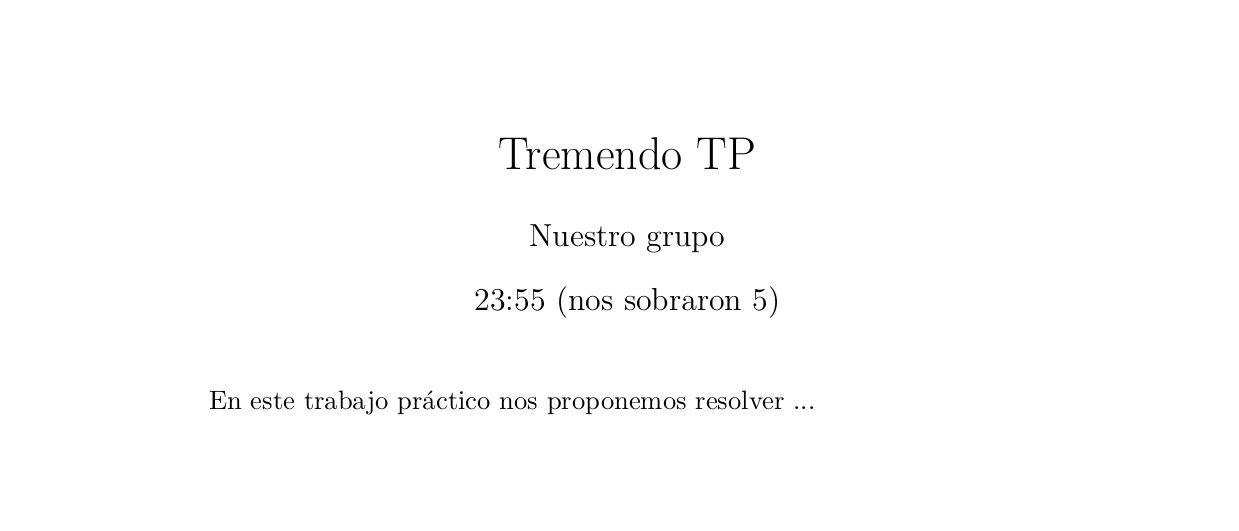
\includegraphics[width=0.9\textwidth]{../images/ejemplo_tp_1.png}
\end{figure}

A su vez, se puede incluir un subtítulo, omitir algunos de los campos, o también usar funciones como \texttt{\textbackslash today} para que la fecha se actualice automáticamente con cada compilación.

\end{frame}

\begin{frame}[containsverbatim]
\frametitle{Ejemplos}
\framesubtitle{Presentaciones}

¿Y si queremos armar slides para una presentación?

\begin{lstlisting}
\documentclass{beamer}
\begin{document}

\begin{frame}[containsverbatim]
\frametitle{Ejemplos}
\framesubtitle{Presentaciones}

¿Y si queremos armar slides para una presentación?

...

\end{frame}

\end{document}
\end{lstlisting}

\end{frame}

\begin{frame}
\frametitle{Ejemplos}
\framesubtitle{Paquetes}

En muchas ocasiones, vamos a querer funcionalidades, entornos, estilos, fuentes, etc. que para utilizarse requieren que usemos el \textbf{paquete} adecuado para ello.

\

Por ejemplo, nos gustaría poder incluir hypervínculos en nuestro documento, de forma que en el contenido del mismo utilice enlaces para acceder a otros documentos o sitios web.
\end{frame}

\begin{frame}
\frametitle{Ejemplos}
\framesubtitle{Paquetes}

Por defecto, tenemos la posibilidad de indicar que algo es una URL. 

Por ejemplo:

\

\begin{center}
\textit{(...)} para más información, consultar la web del departamento de compuntación \url{https://www.dc.uba.ar}.
\end{center}

\pause

Mientras que utilizando el paquete \href{https://ctan.org/pkg/hyperref}{hyperref} podemos escribir lo siguiente


\begin{center}
\textit{(...)} para más información, consultar la web del \href{https://www.dc.uba.ar}{departamento de computación}.
\end{center}

Lo cual resulta más prolijo para enlazar URLs, secciones de un informe, referencias, etc.

\end{frame}
